\documentclass[../main.tex]{subfiles}

\begin{document}

These plots show a graphical visualisation of change point detections when change point detection algorithms are applied to real-world data sets. Algorithms detecting changes in \emph{mean} show horizontal red bars at the current mean between change points, while algorithms detecting changes in \emph{variance} or \emph{mean \& variance} show the change points as vertical red bars. The \emph{ground truth} is indicated by a vertical dashed blue line.

\begin{figure}[h]
    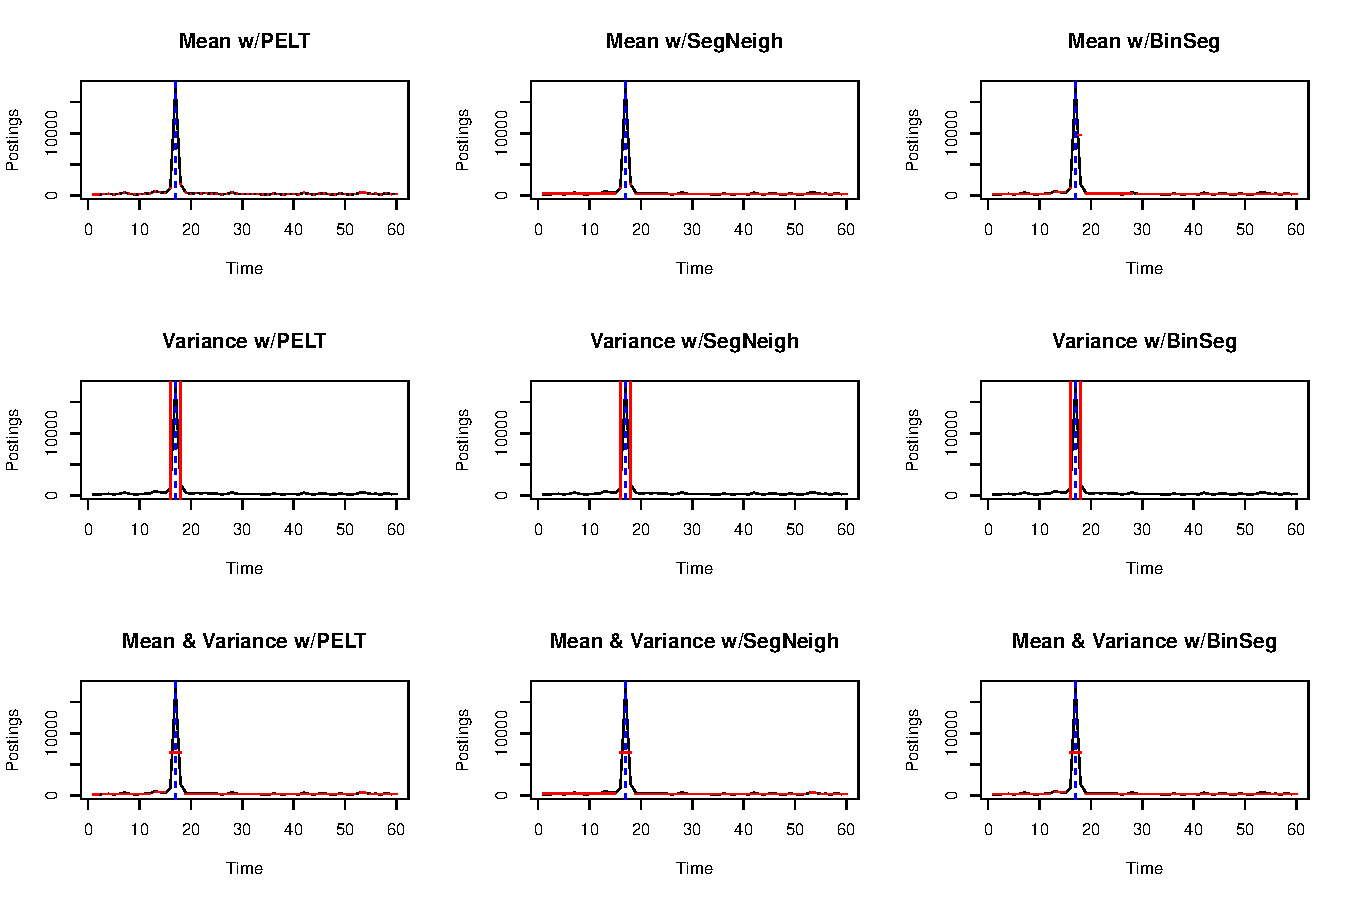
\includegraphics[width=\textwidth]{figures/dirkresults}
    \caption{`Dirk' Change Point Detections}
    \label{fig:dirk}
\end{figure}

\begin{figure}[h]
    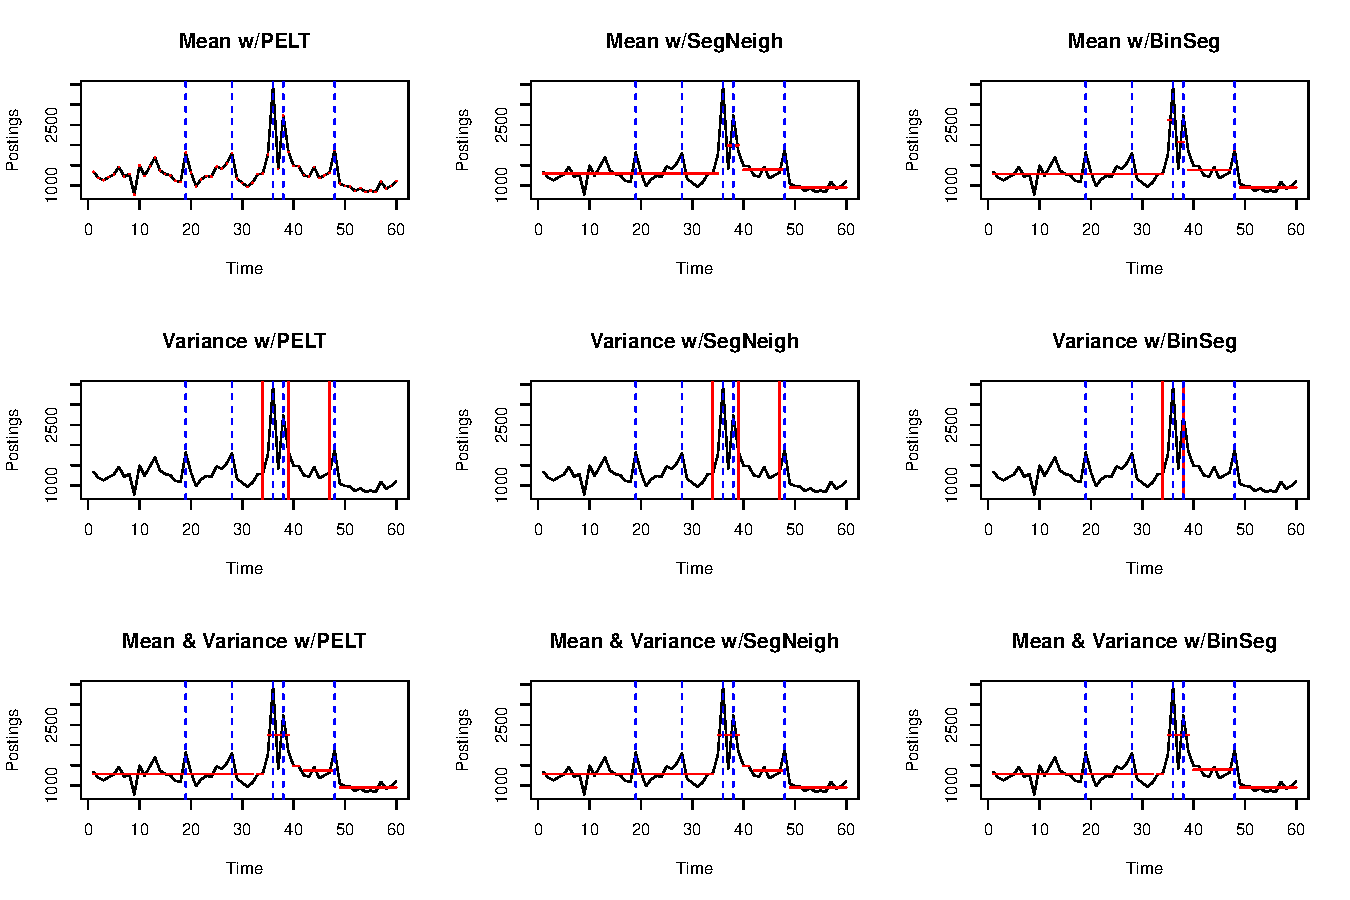
\includegraphics[width=\textwidth]{figures/ziggoresults}
    \caption{`Ziggo' Change Point Detections}
    \label{fig:ziggo}
\end{figure}


\begin{figure}[h]
    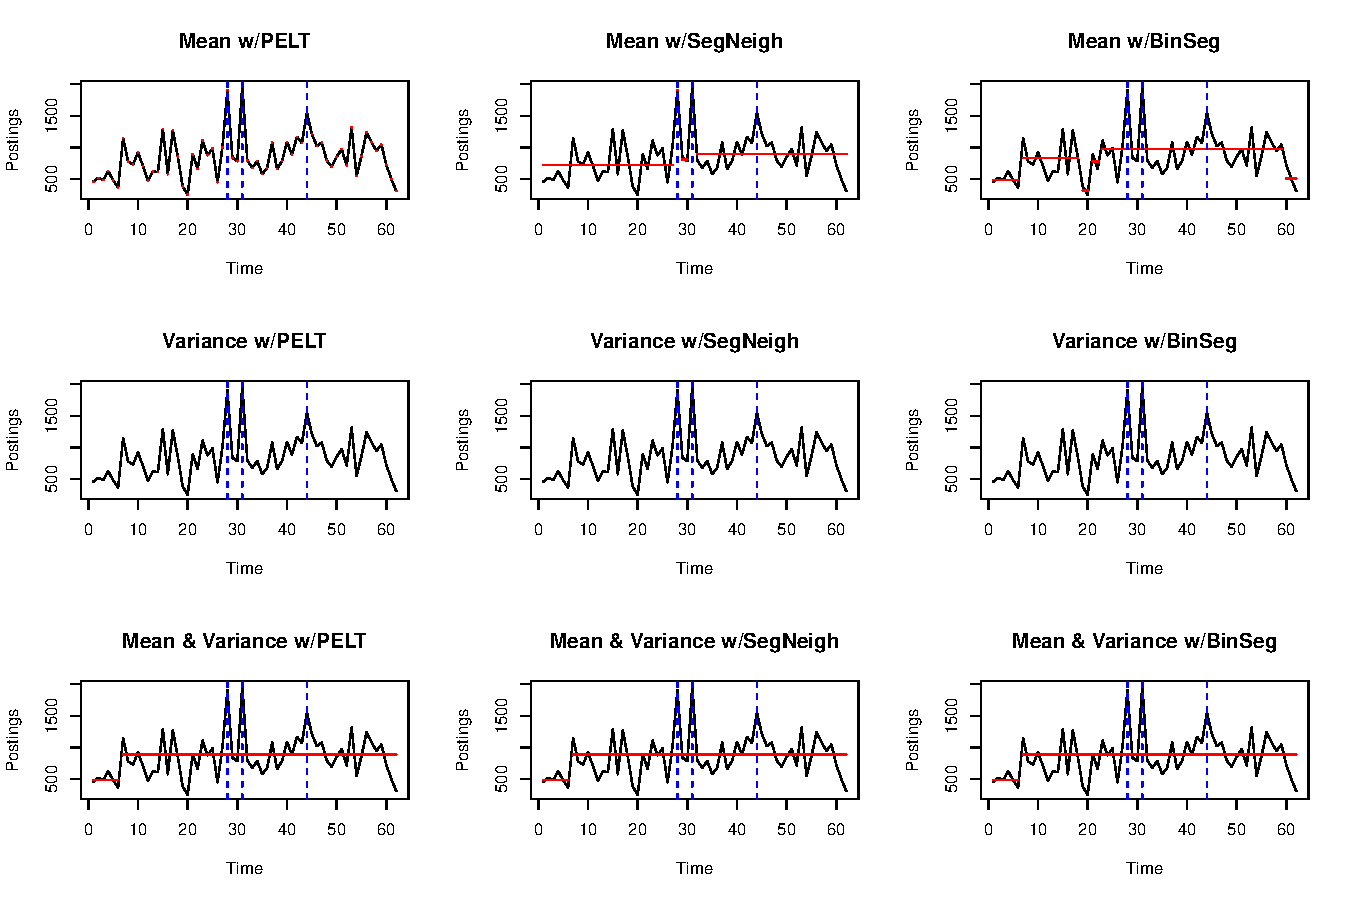
\includegraphics[width=\textwidth]{figures/bolresults}
    \caption{`Bol.com' Change Point Detections}
    \label{fig:bol}
\end{figure}


\begin{figure}[h]
    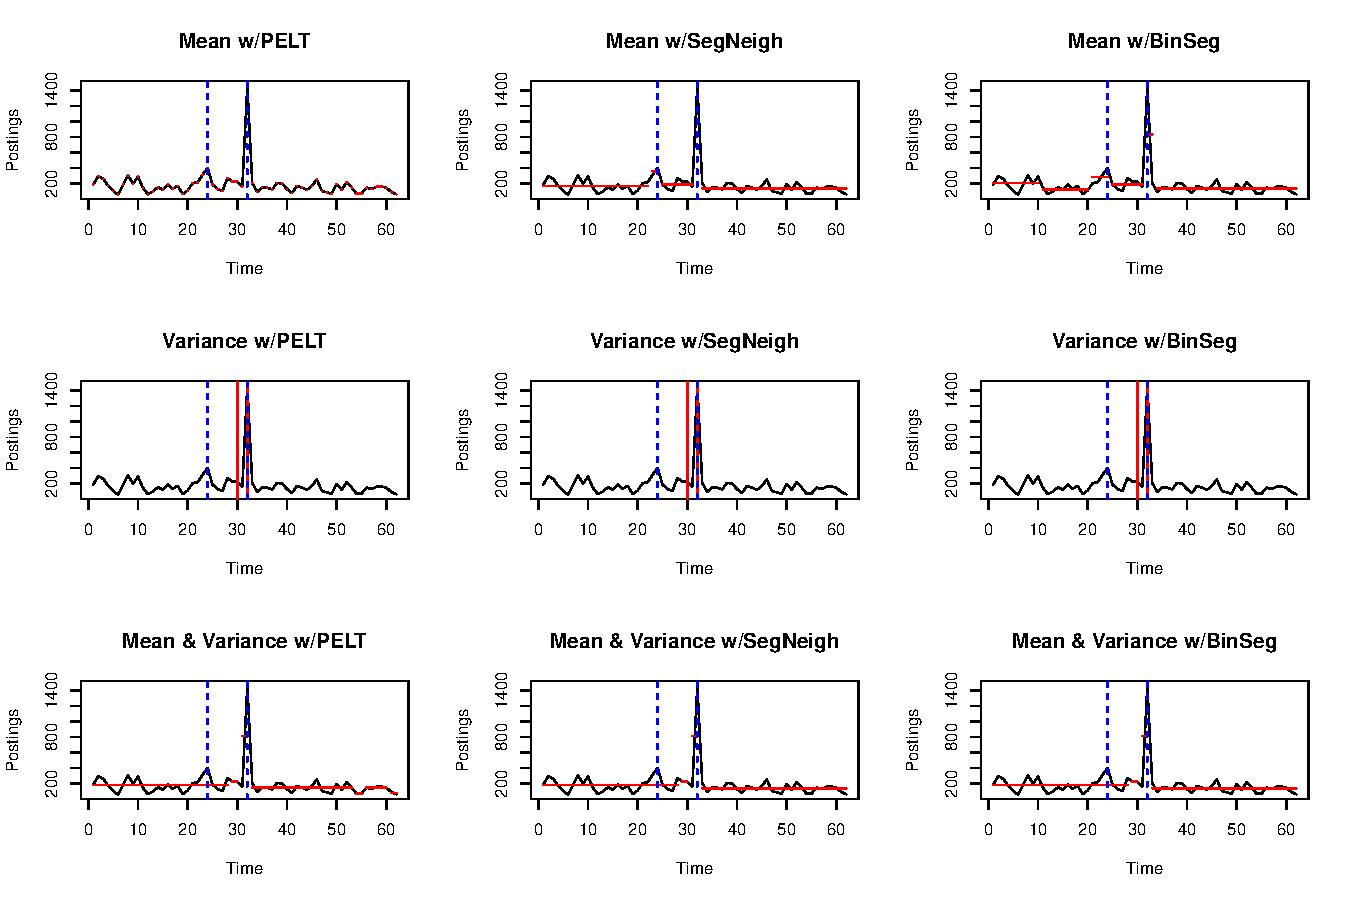
\includegraphics[width=\textwidth]{figures/connexxionresults}
    \caption{`Connexxion' Change Point Detections}
    \label{fig:connexxion}
\end{figure}

\begin{figure}[h]
    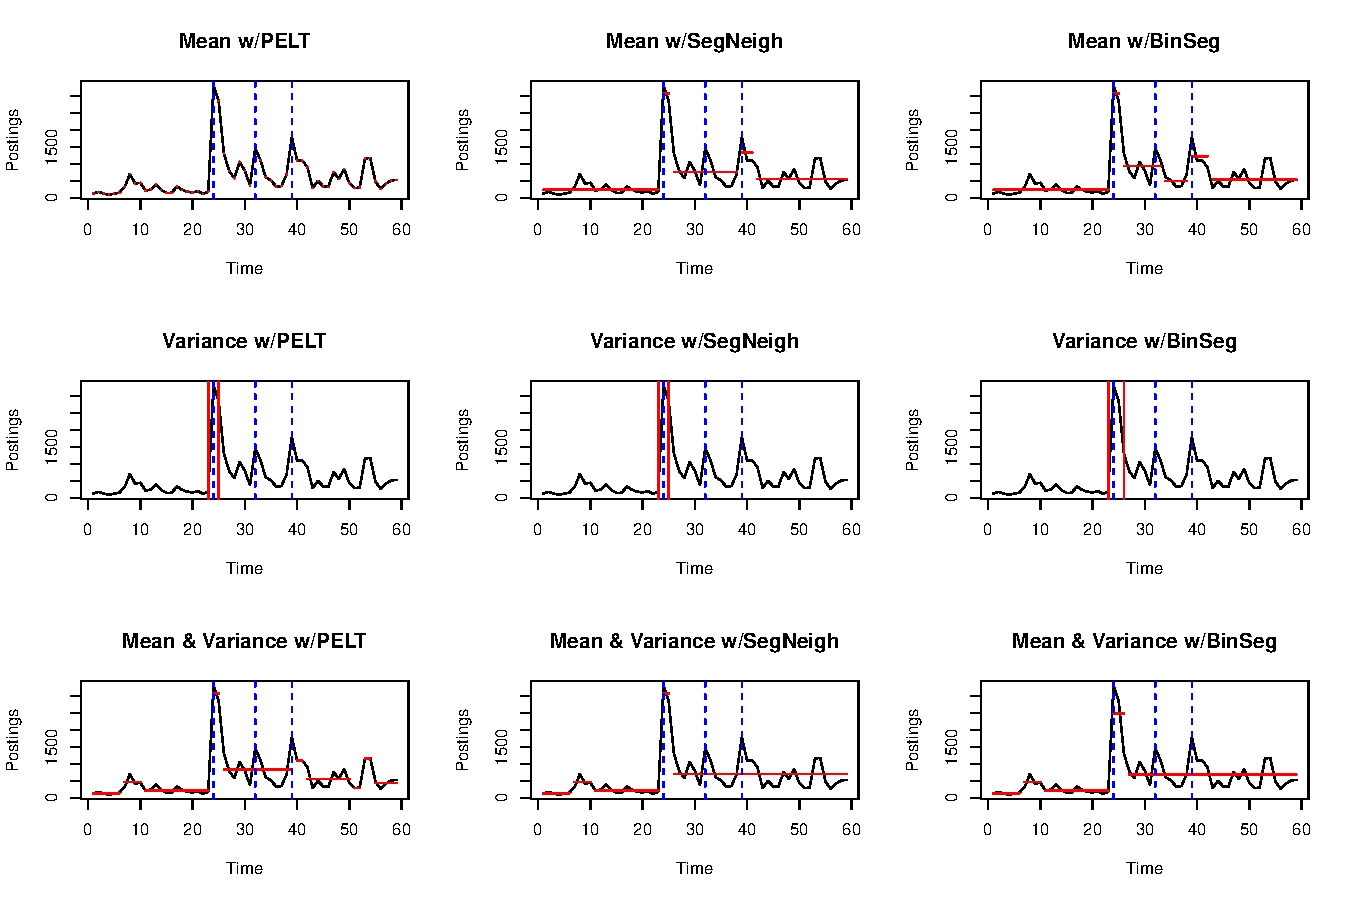
\includegraphics[width=\textwidth]{figures/dapresults}
    \caption{`Dakota Access Pipeline' Change Point Detections}
    \label{fig:dap}
\end{figure}

\begin{figure}[h]
    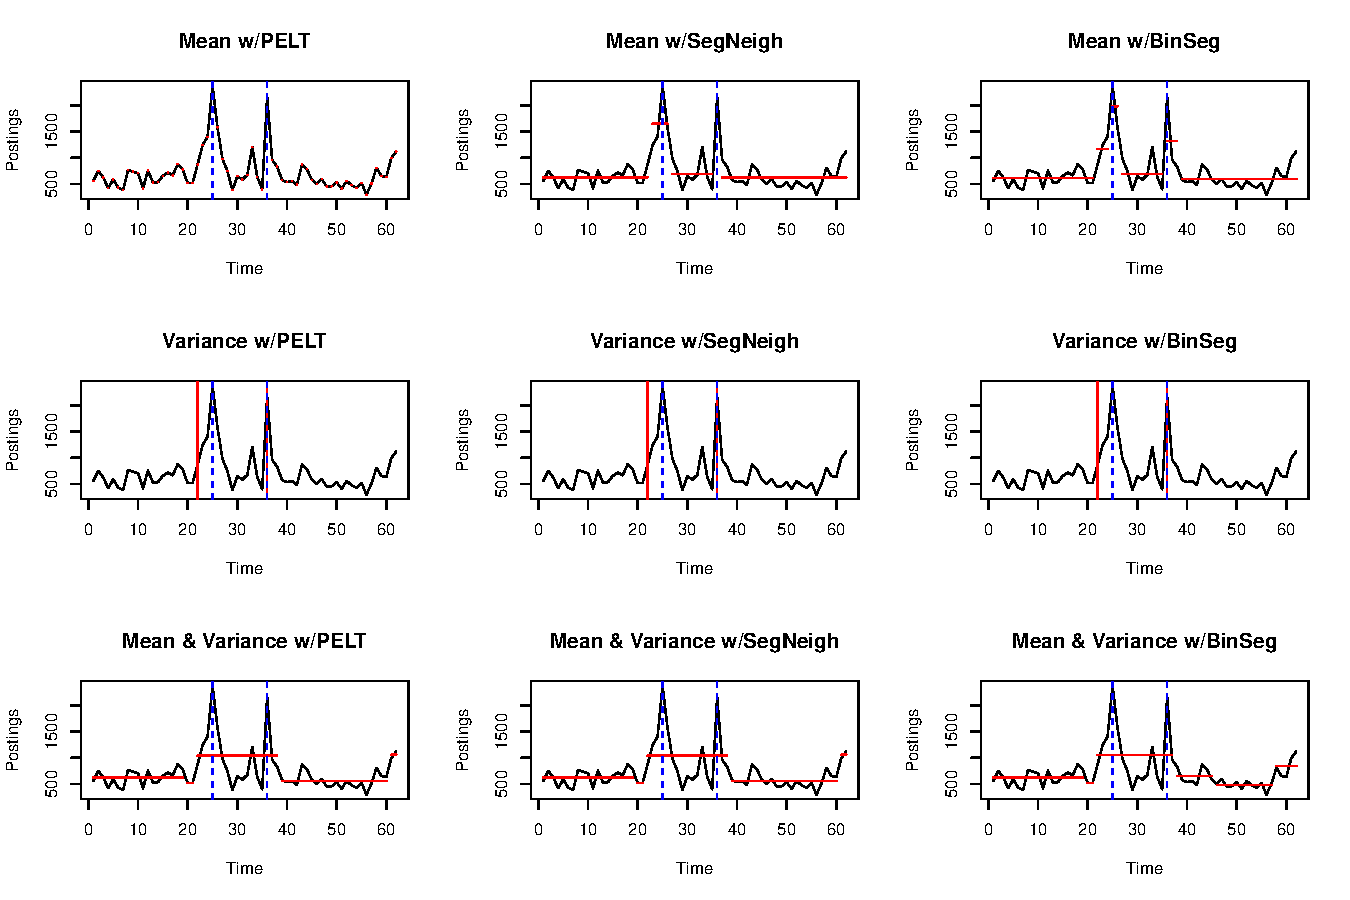
\includegraphics[width=\textwidth]{figures/jumboresults}
    \caption{`Jumbo' Change Point Detections}
    \label{fig:jumbo}
\end{figure}

\begin{figure}[h]
    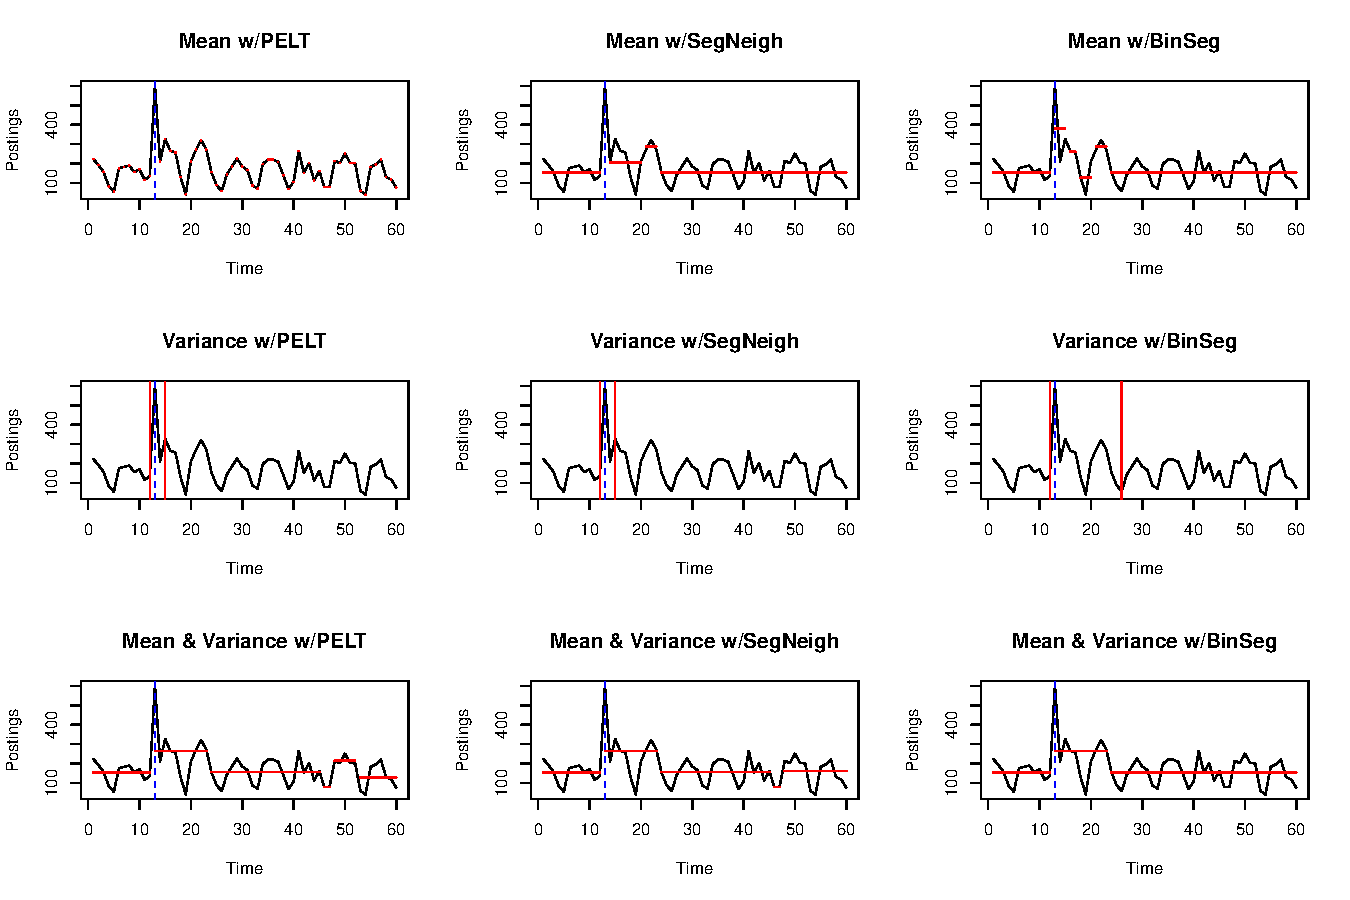
\includegraphics[width=\textwidth]{figures/kvkresults}
    \caption{`Kamer van Koophandel' Change Point Detections}
    \label{fig:kvk}
\end{figure}

\begin{figure}[h]
    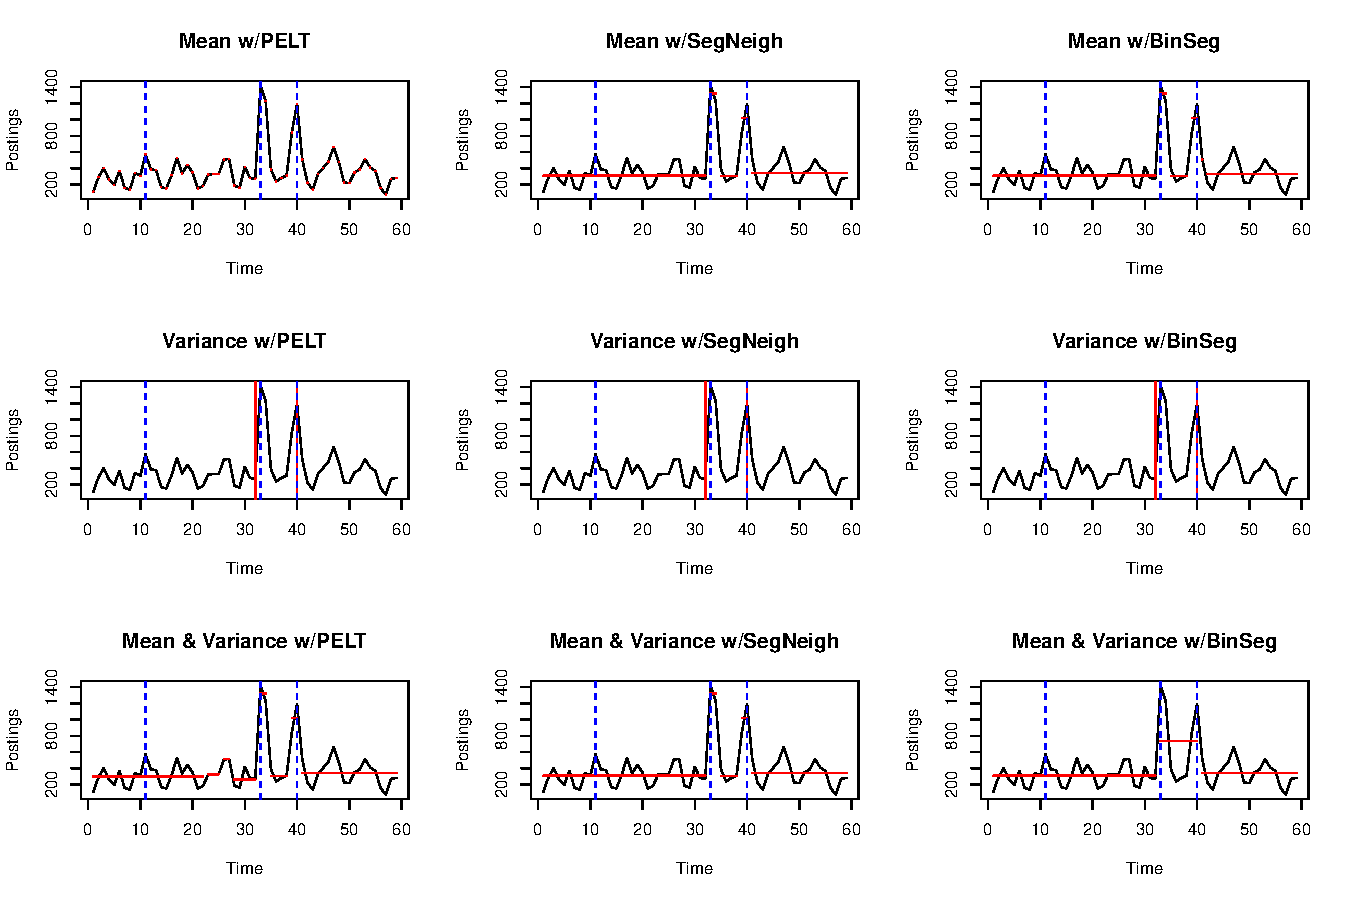
\includegraphics[width=\textwidth]{figures/rabobankresults}
    \caption{`Rabobank' Change Point Detections}
    \label{fig:rabobank}
\end{figure}


\begin{figure}[h]
    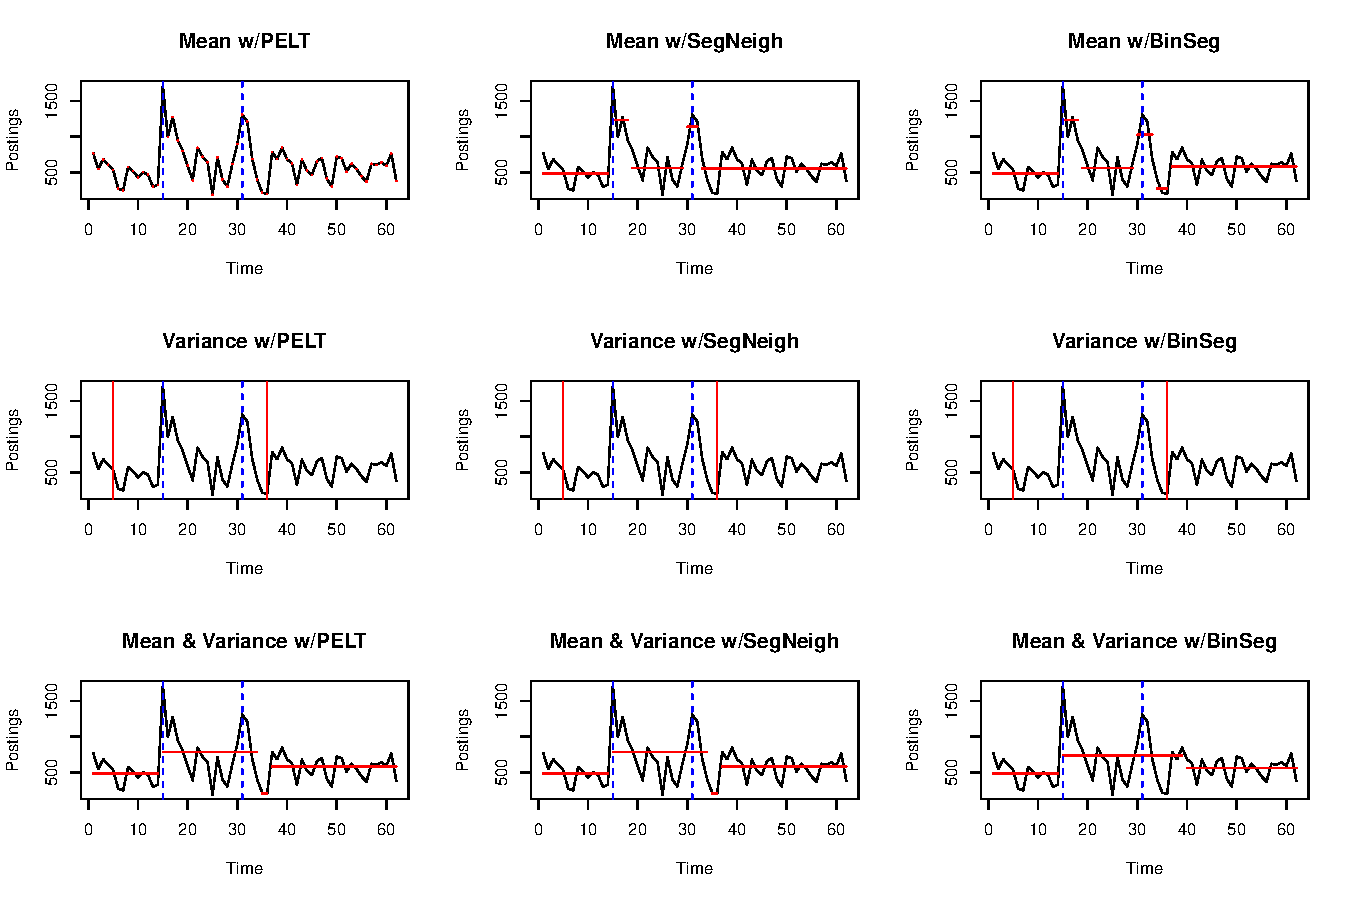
\includegraphics[width=\textwidth]{figures/tele2results}
    \caption{`Tele2' Change Point Detections}
    \label{fig:tele2}
\end{figure}


\begin{figure}[h]
    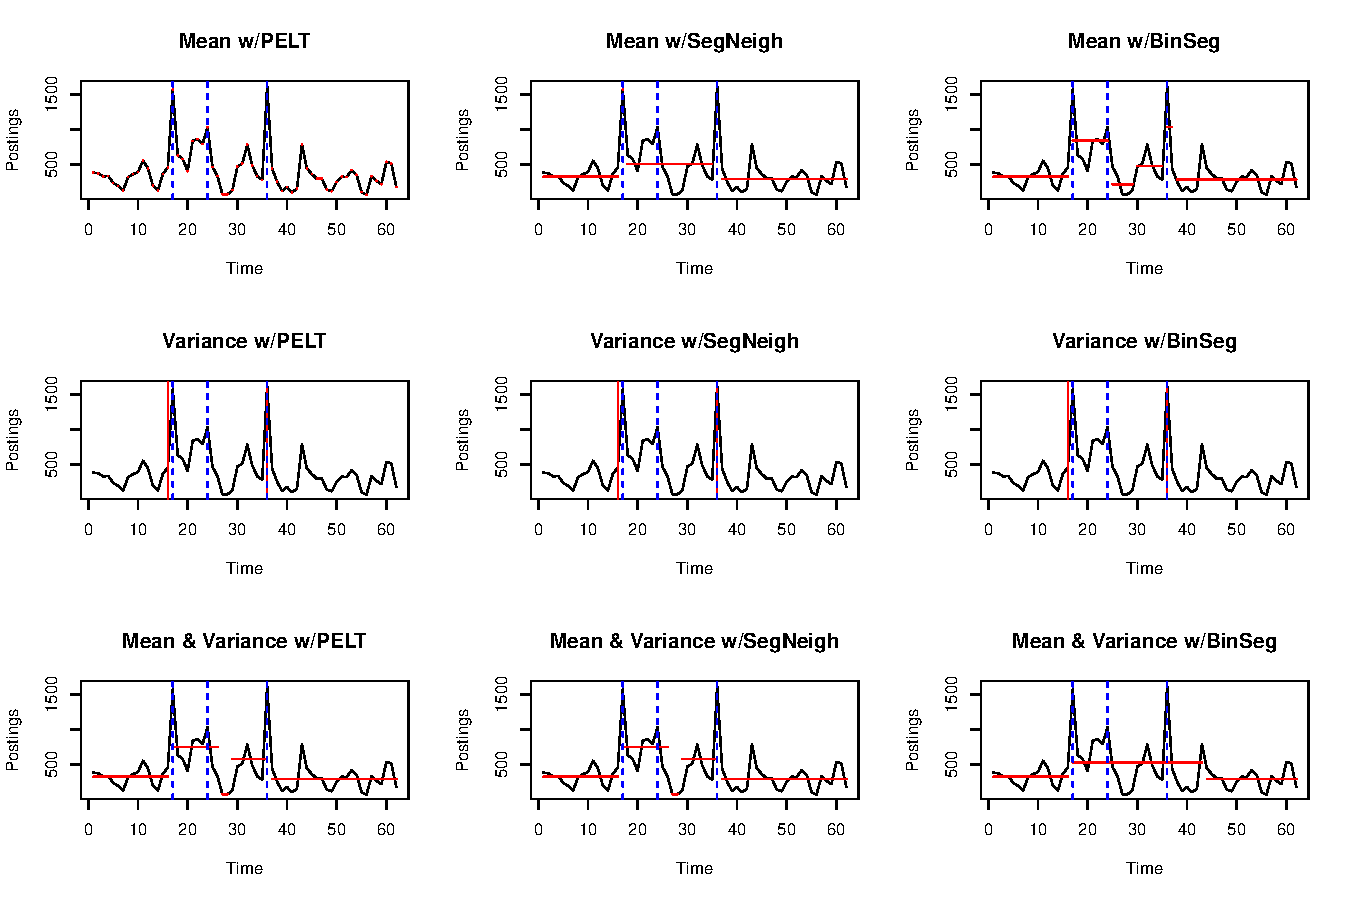
\includegraphics[width=\textwidth]{figures/uwvresults}
    \caption{`UWV' Change Point Detections}
    \label{fig:uwv}
\end{figure}

\end{document}